\section{User Interface}

A front-end for the APIs is implemented which provides a graphical user interface for the underlying functionality. Figures \ref{fig:ss1},\ref{fig:ss2},\ref{fig:ss3},\ref{fig:ss4},\ref{fig:ss5},\ref{fig:ss6} and \ref{fig:ss7} show the interface and explain the functionality.

\begin{figure}[!h]
\begin{center}
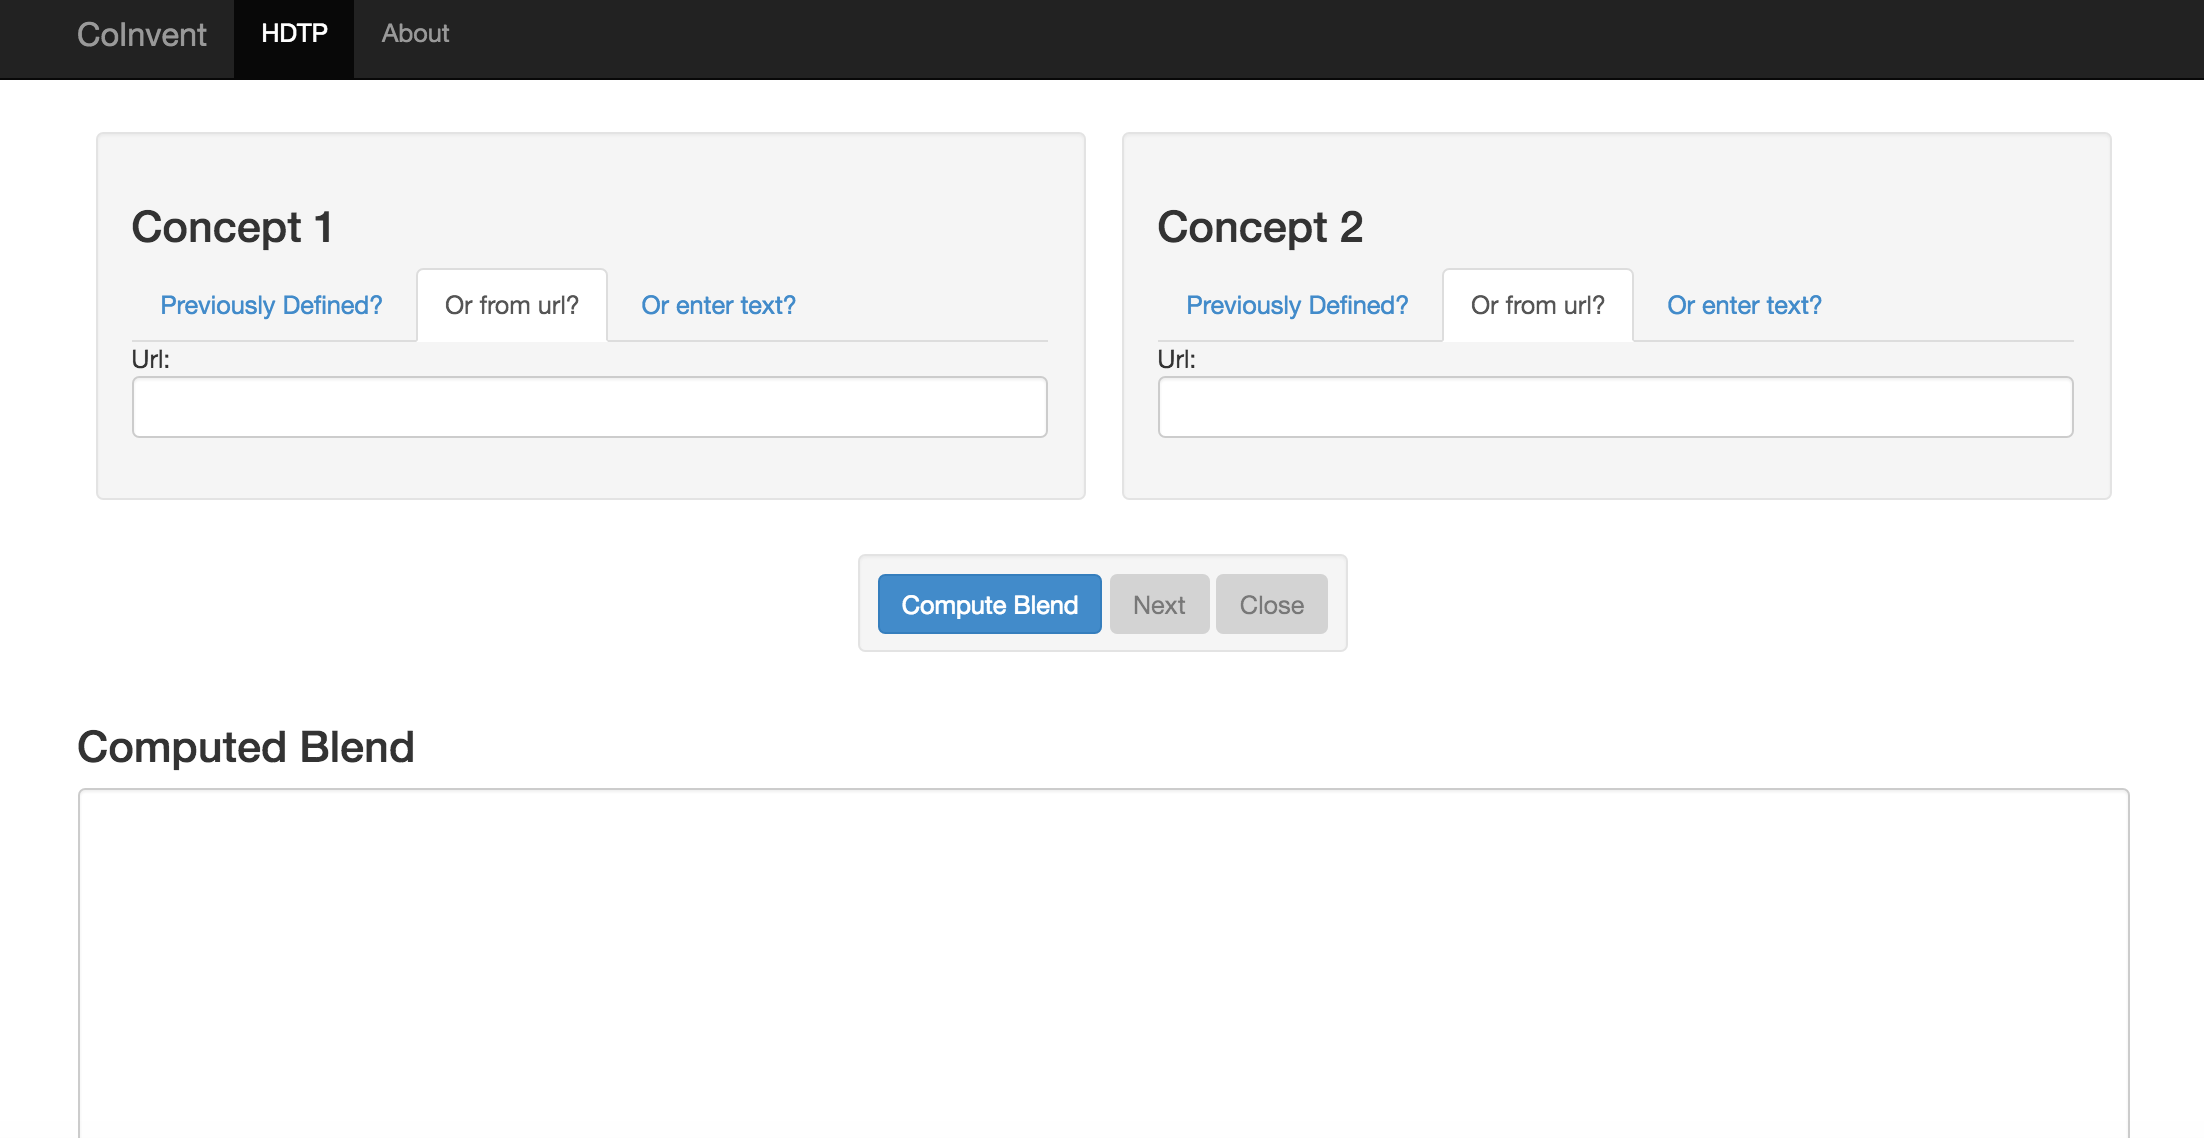
\includegraphics[width=\textwidth]{ss1.png}
\end{center}
\label{fig:ss1}
\caption{The Coinvent system main page, showing the two panes where the input concepts or theories can be selected}
\end{figure}

\begin{figure}[!h]
\begin{center}
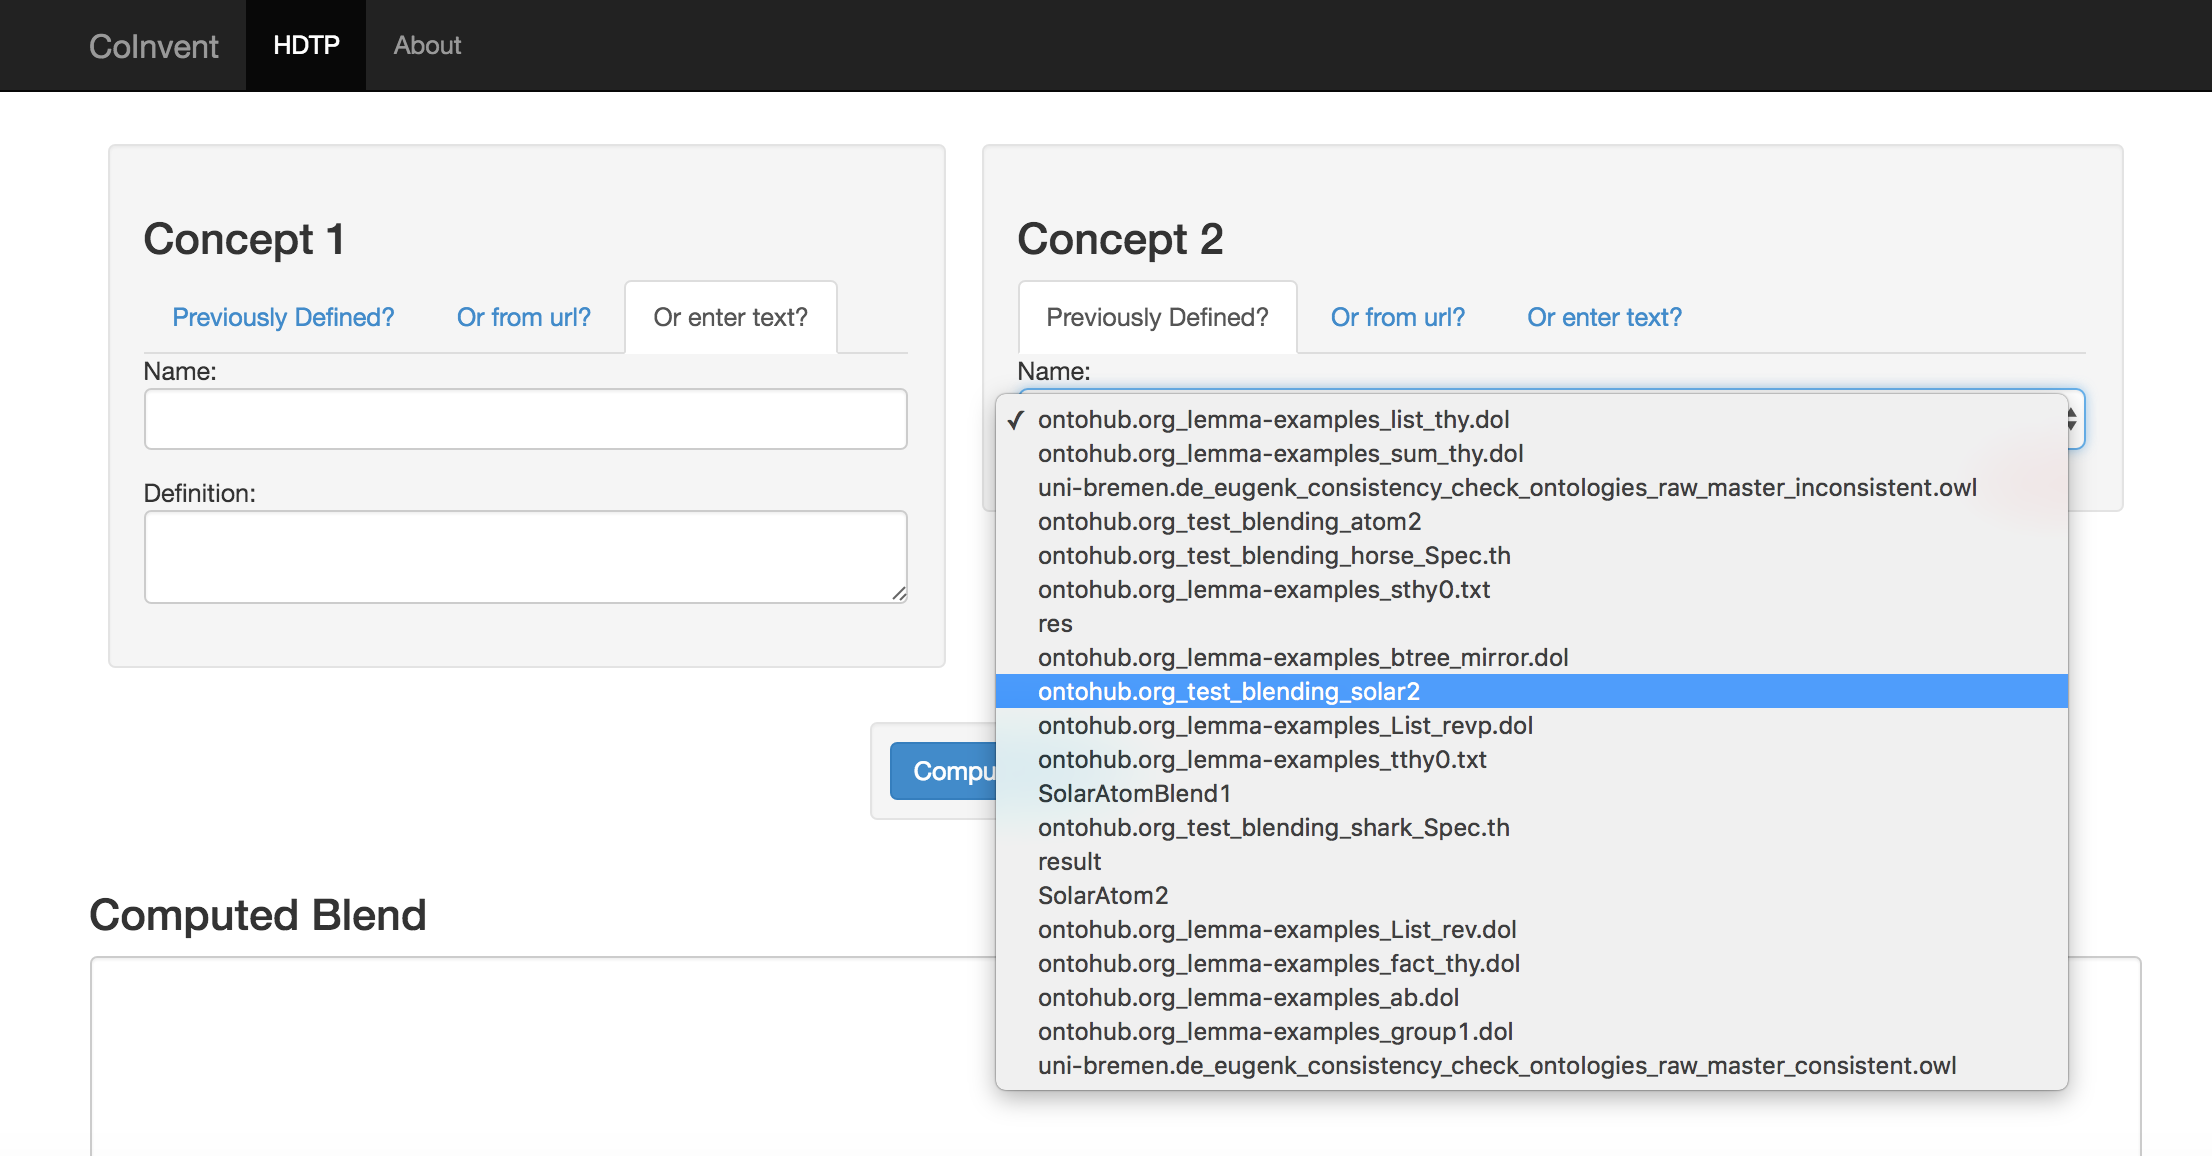
\includegraphics[width=\textwidth]{ss2.png}
\end{center}
\label{fig:ss2}
\caption{The Coinvent system main page, showing how a new theory can be defined in the text area on the left, and how a previous theory can be seleted in the right pane}
\end{figure}

\begin{figure}[!h]
\begin{center}
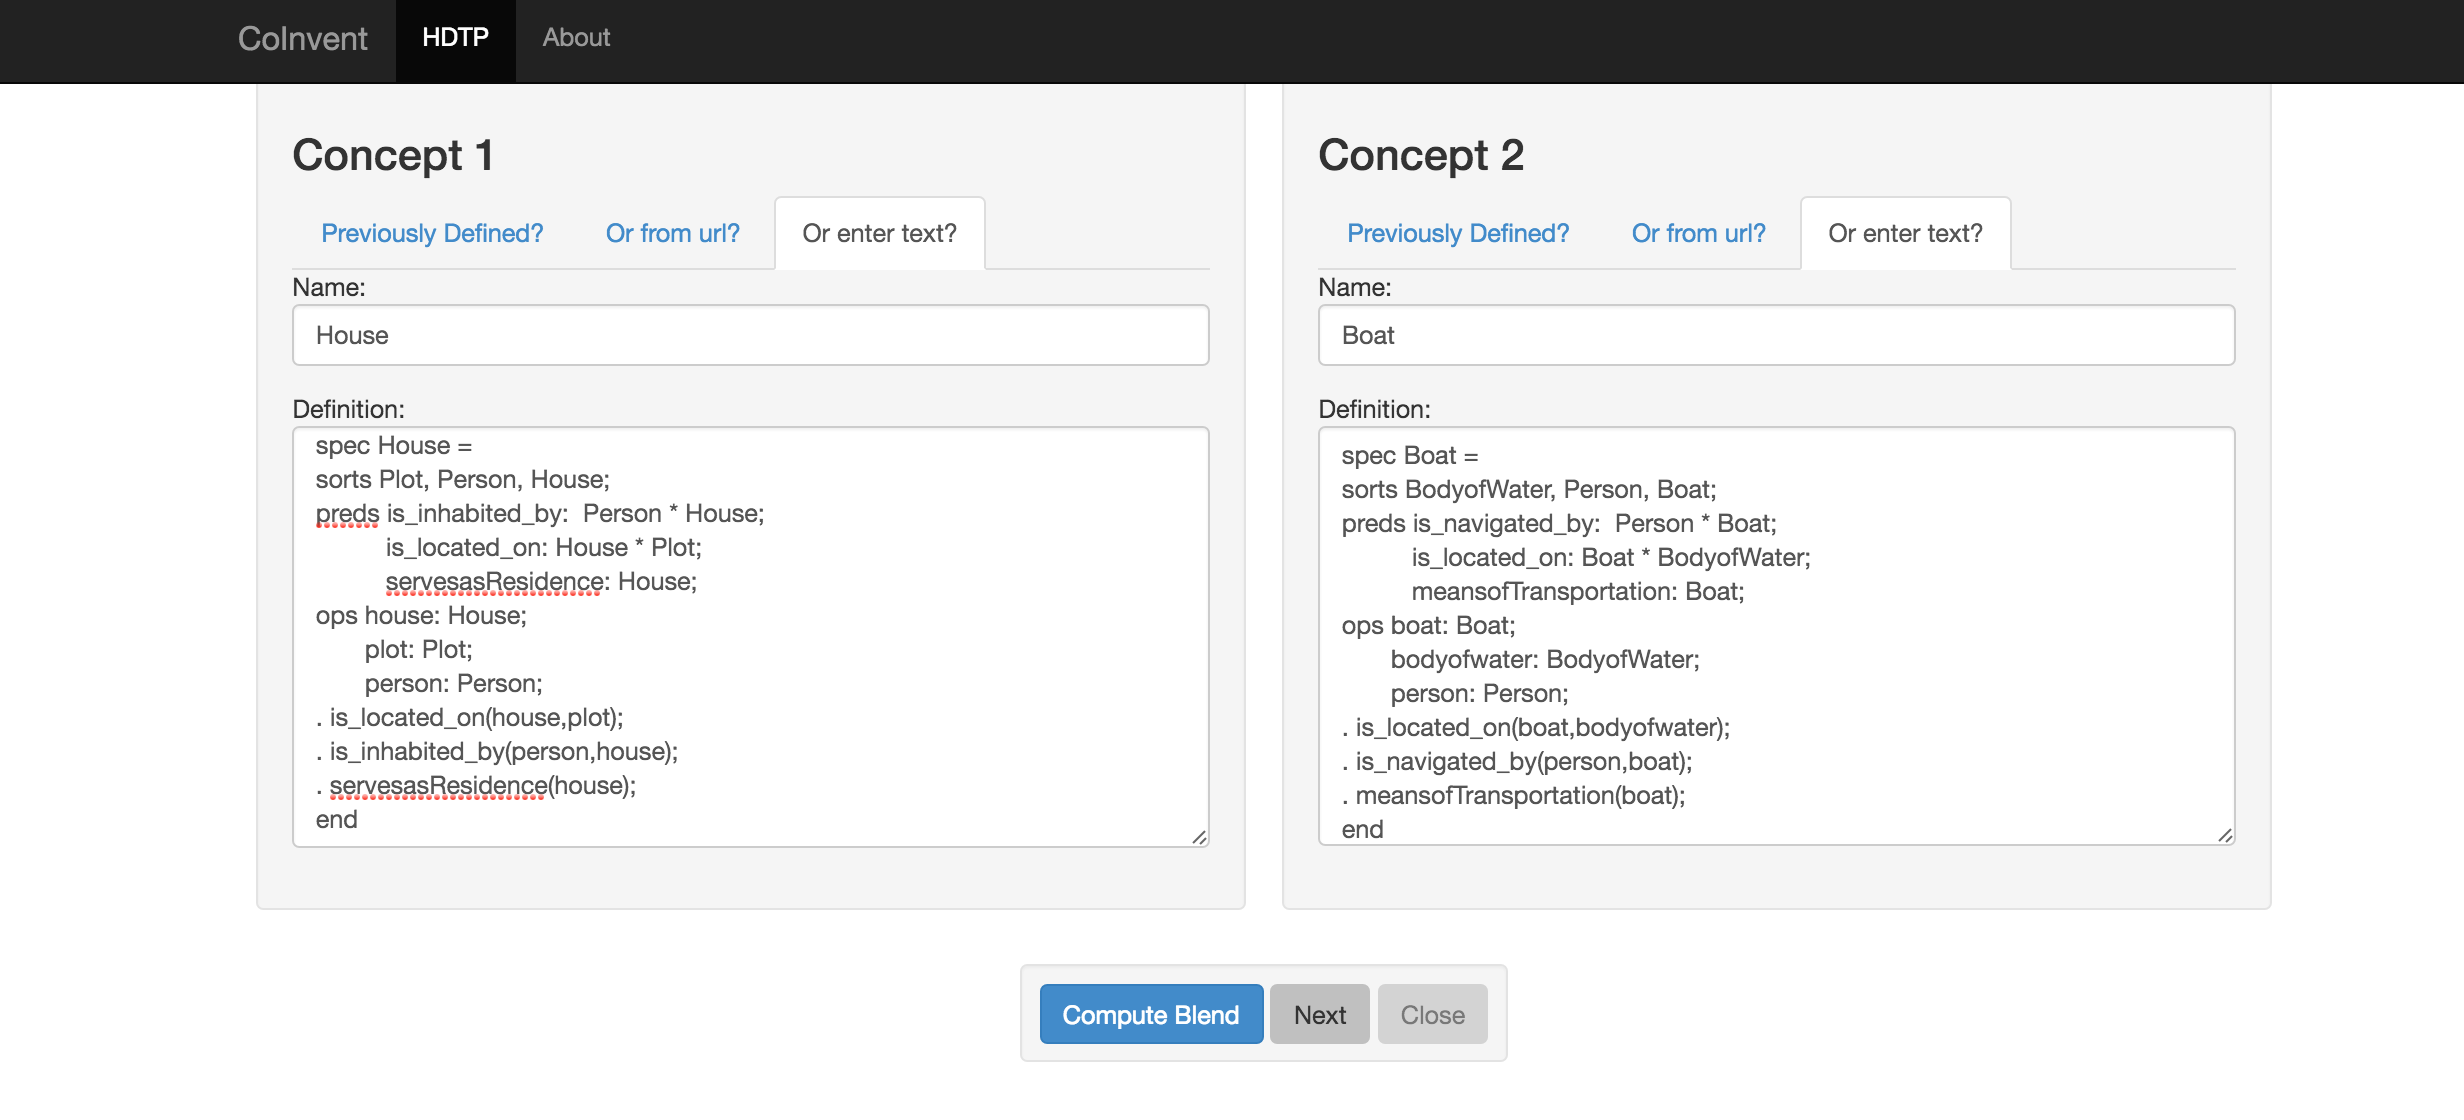
\includegraphics[width=\textwidth]{ss3.png}
\end{center}
\label{fig:ss3}
\caption{Defining new concepts in the text entry box in the Coinvent System}
\end{figure}

\begin{figure}[!h]
\begin{center}
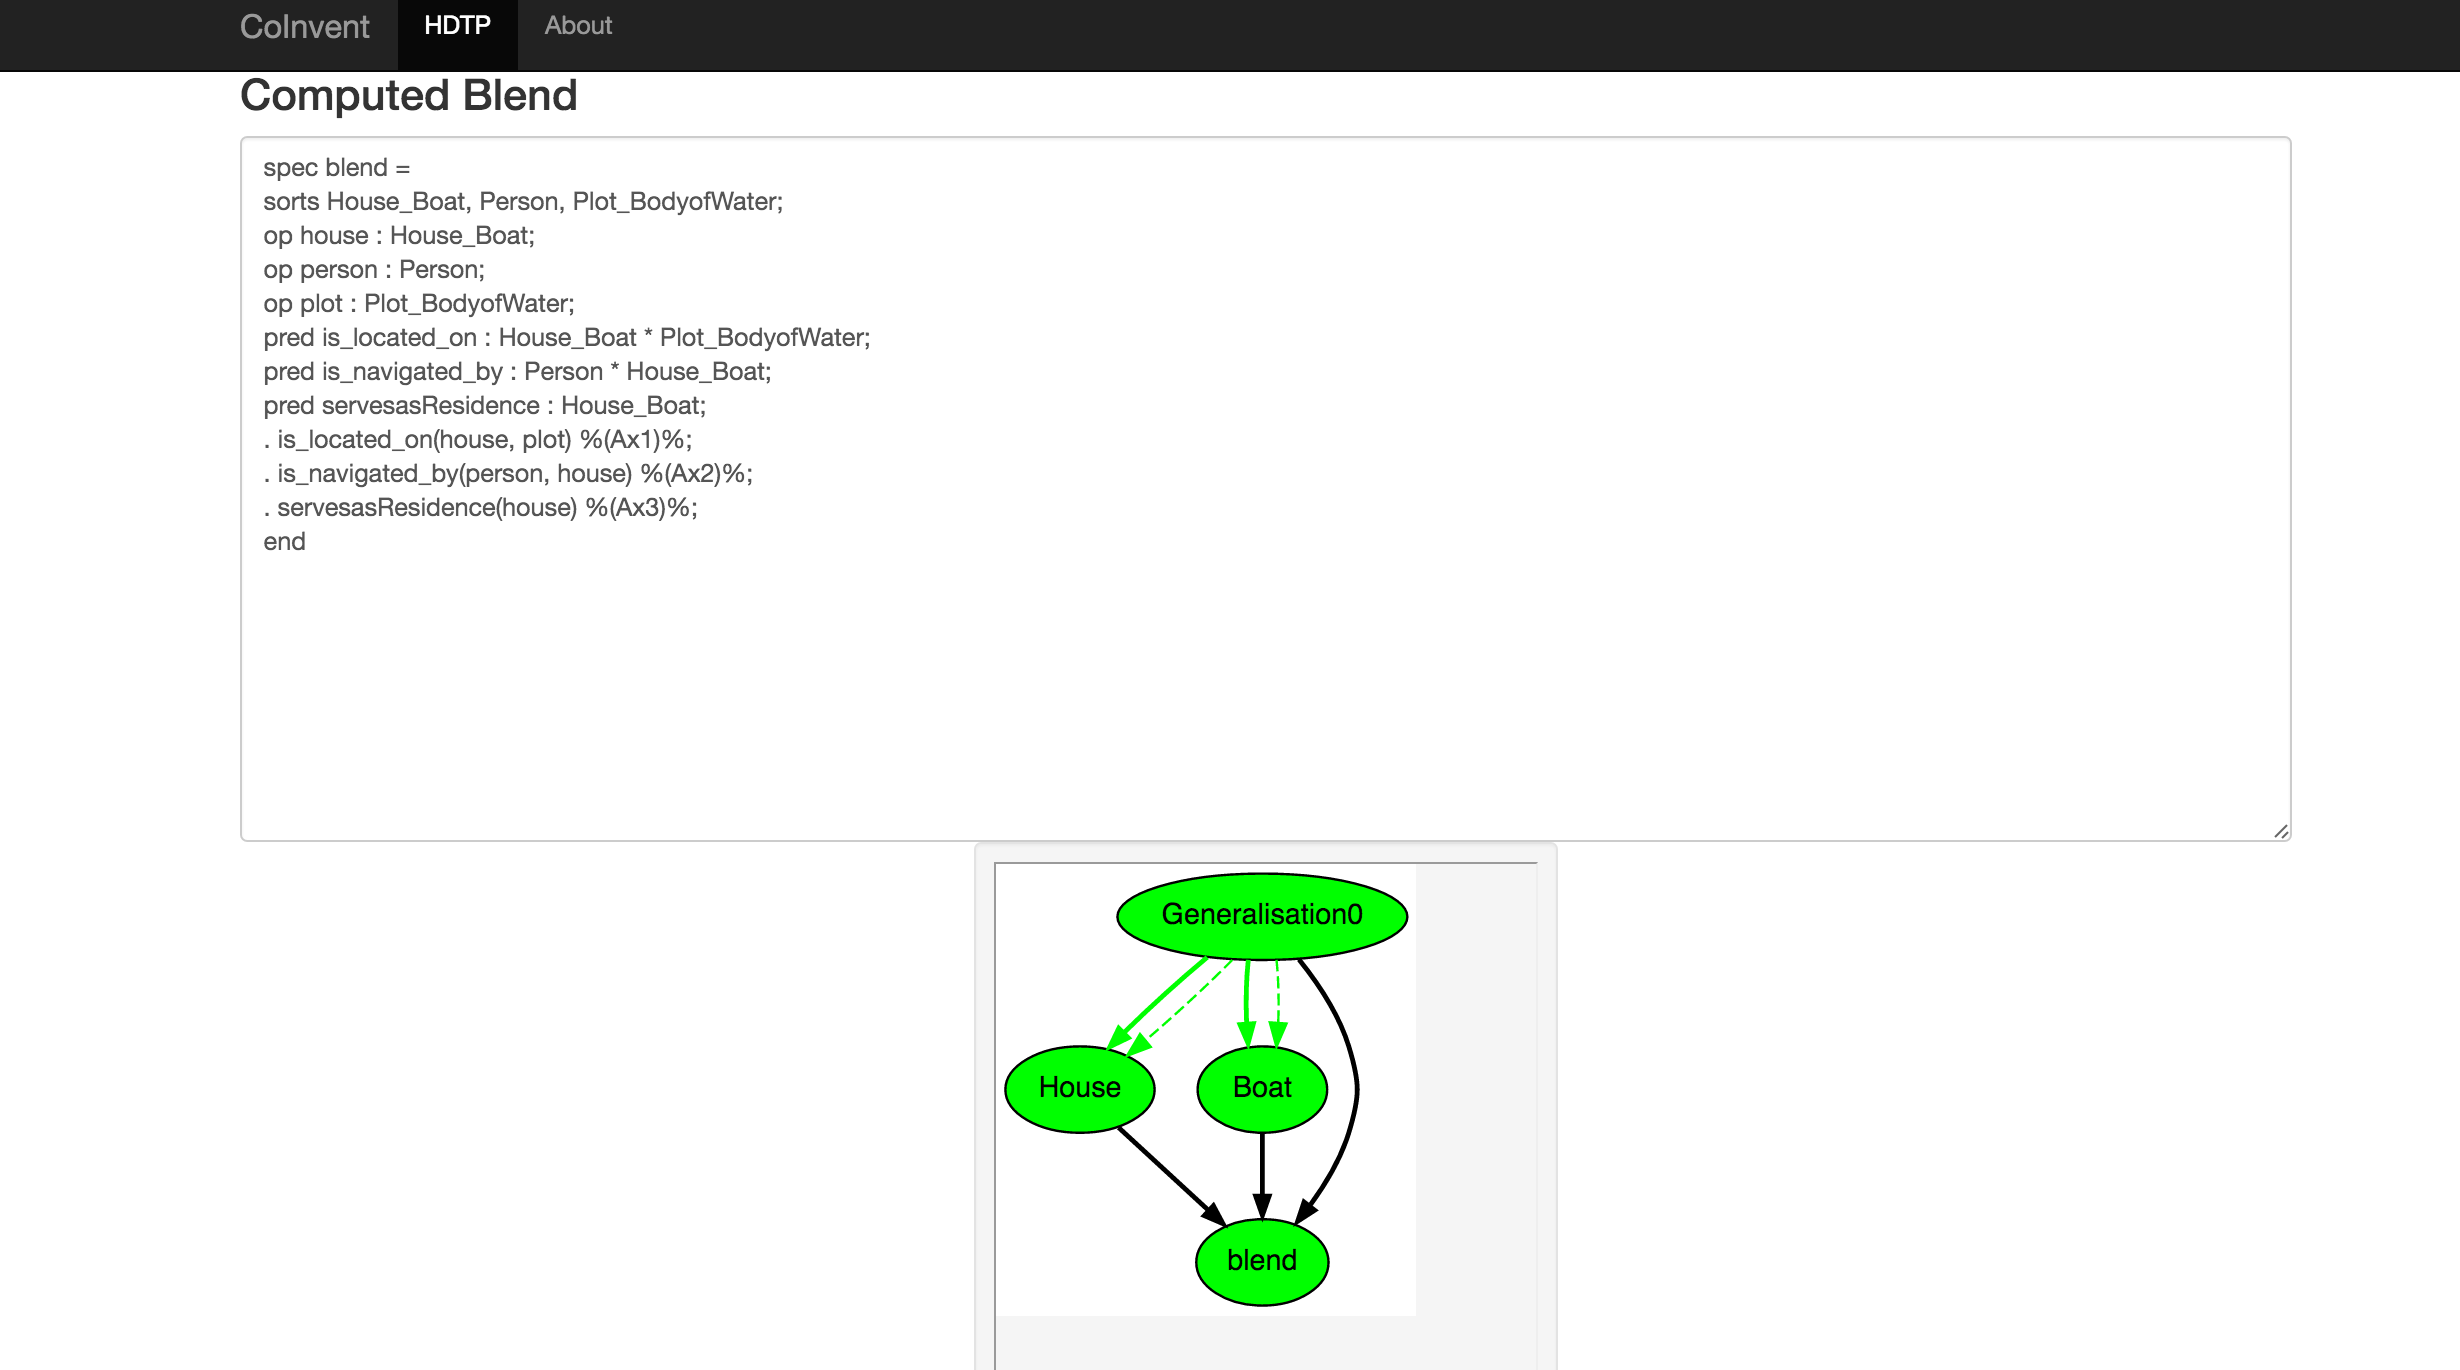
\includegraphics[width=\textwidth]{ss4.png}
\end{center}
\label{fig:ss4}
\caption{The result of computing the blend in the Coinvent System showing the graphical and text depiction of the blend}
\end{figure}

\begin{figure}[!h]
\begin{center}
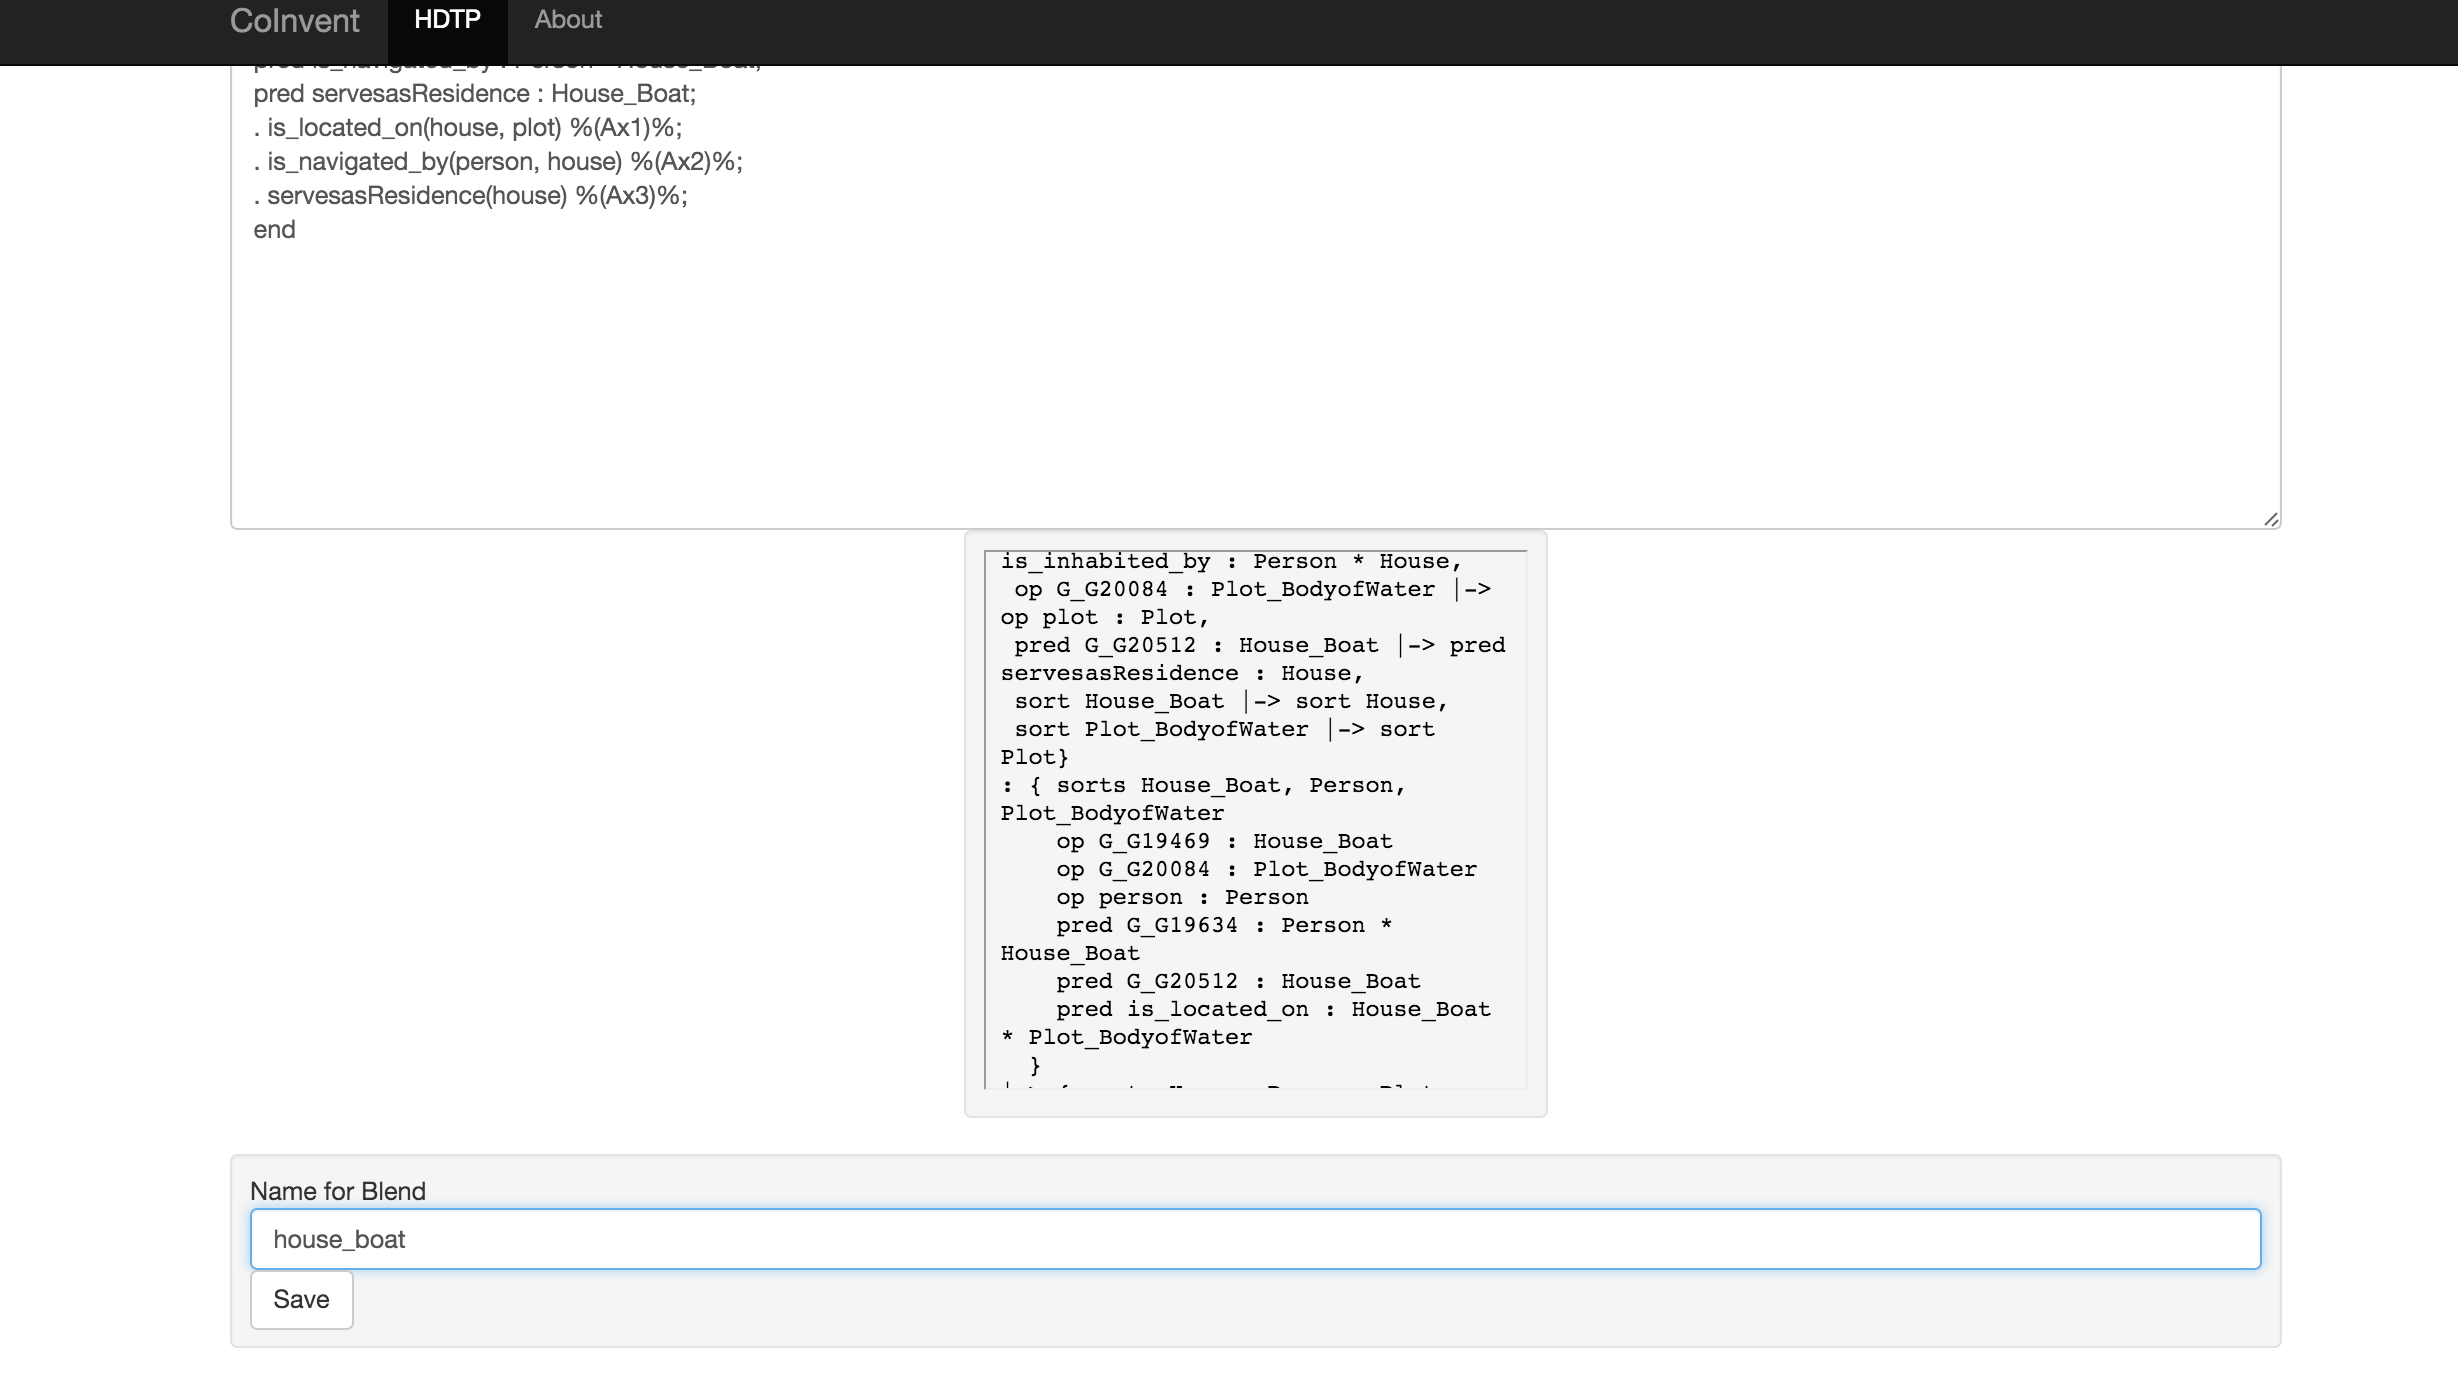
\includegraphics[width=\textwidth]{ss5.png}
\end{center}
\label{fig:ss5}
\caption{Investigating the calculated morphisms and saving the resulting blend}
\end{figure}

\begin{figure}[!h]
\begin{center}
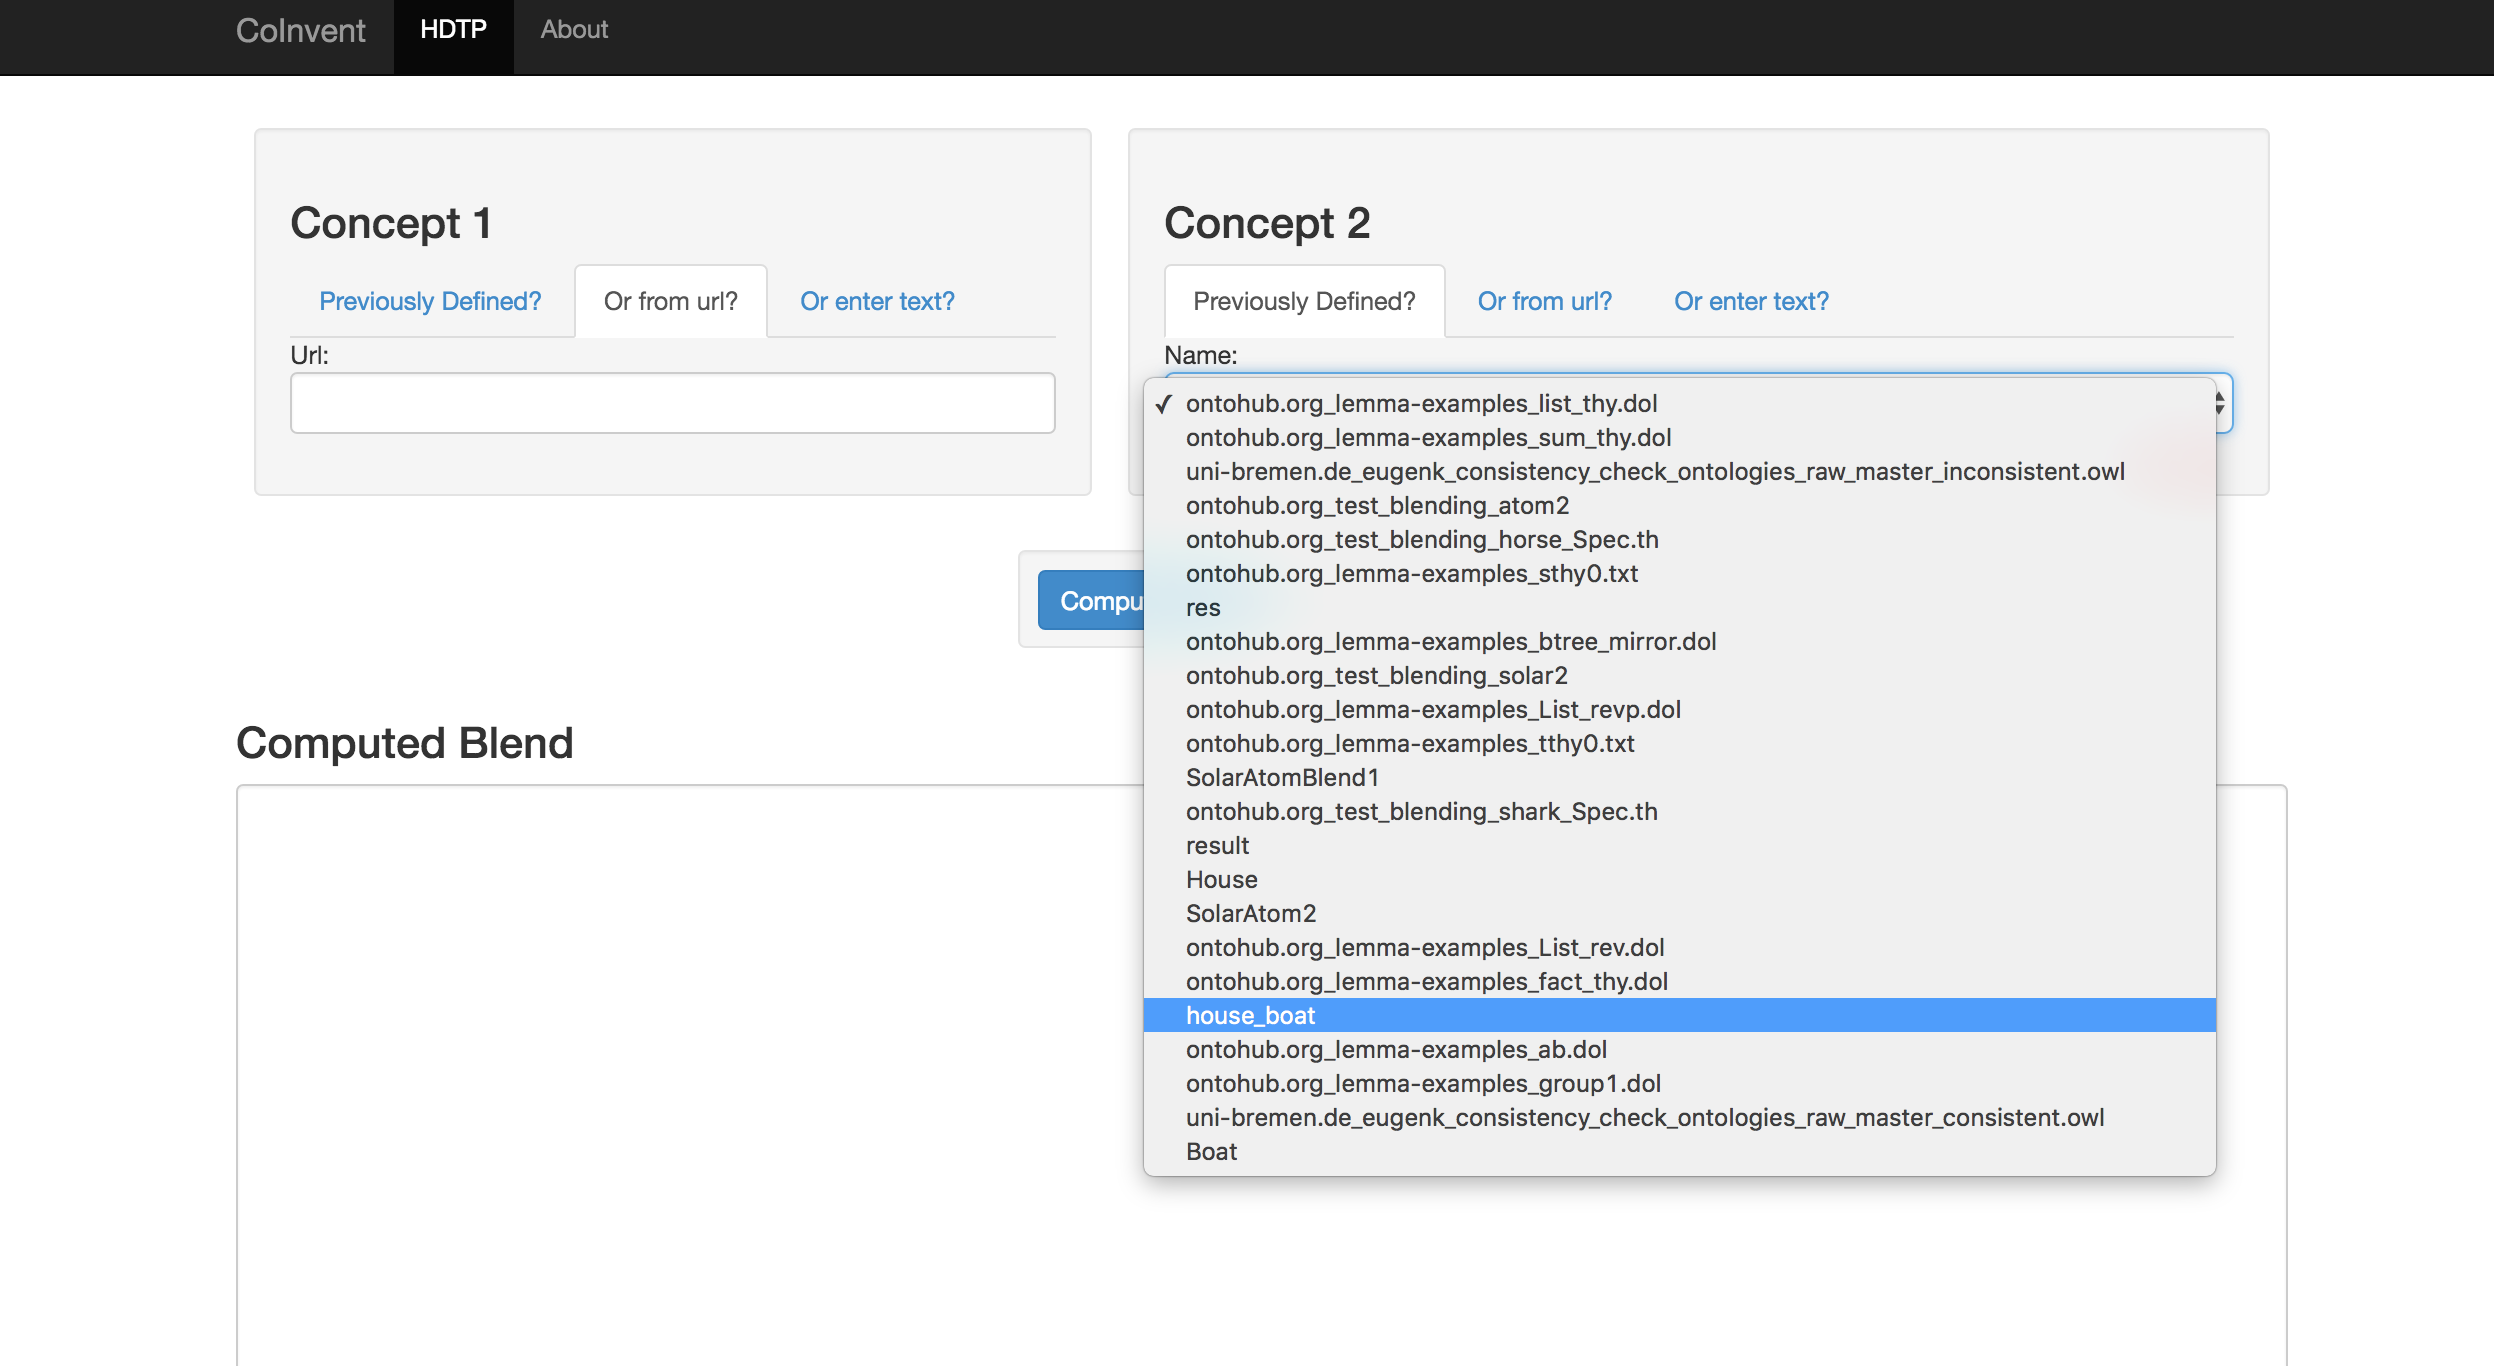
\includegraphics[width=\textwidth]{ss6.png}
\end{center}
\label{fig:ss6}
\caption{Selecting a saved blend as an input theory}
\end{figure}

\begin{figure}[!h]
\begin{center}
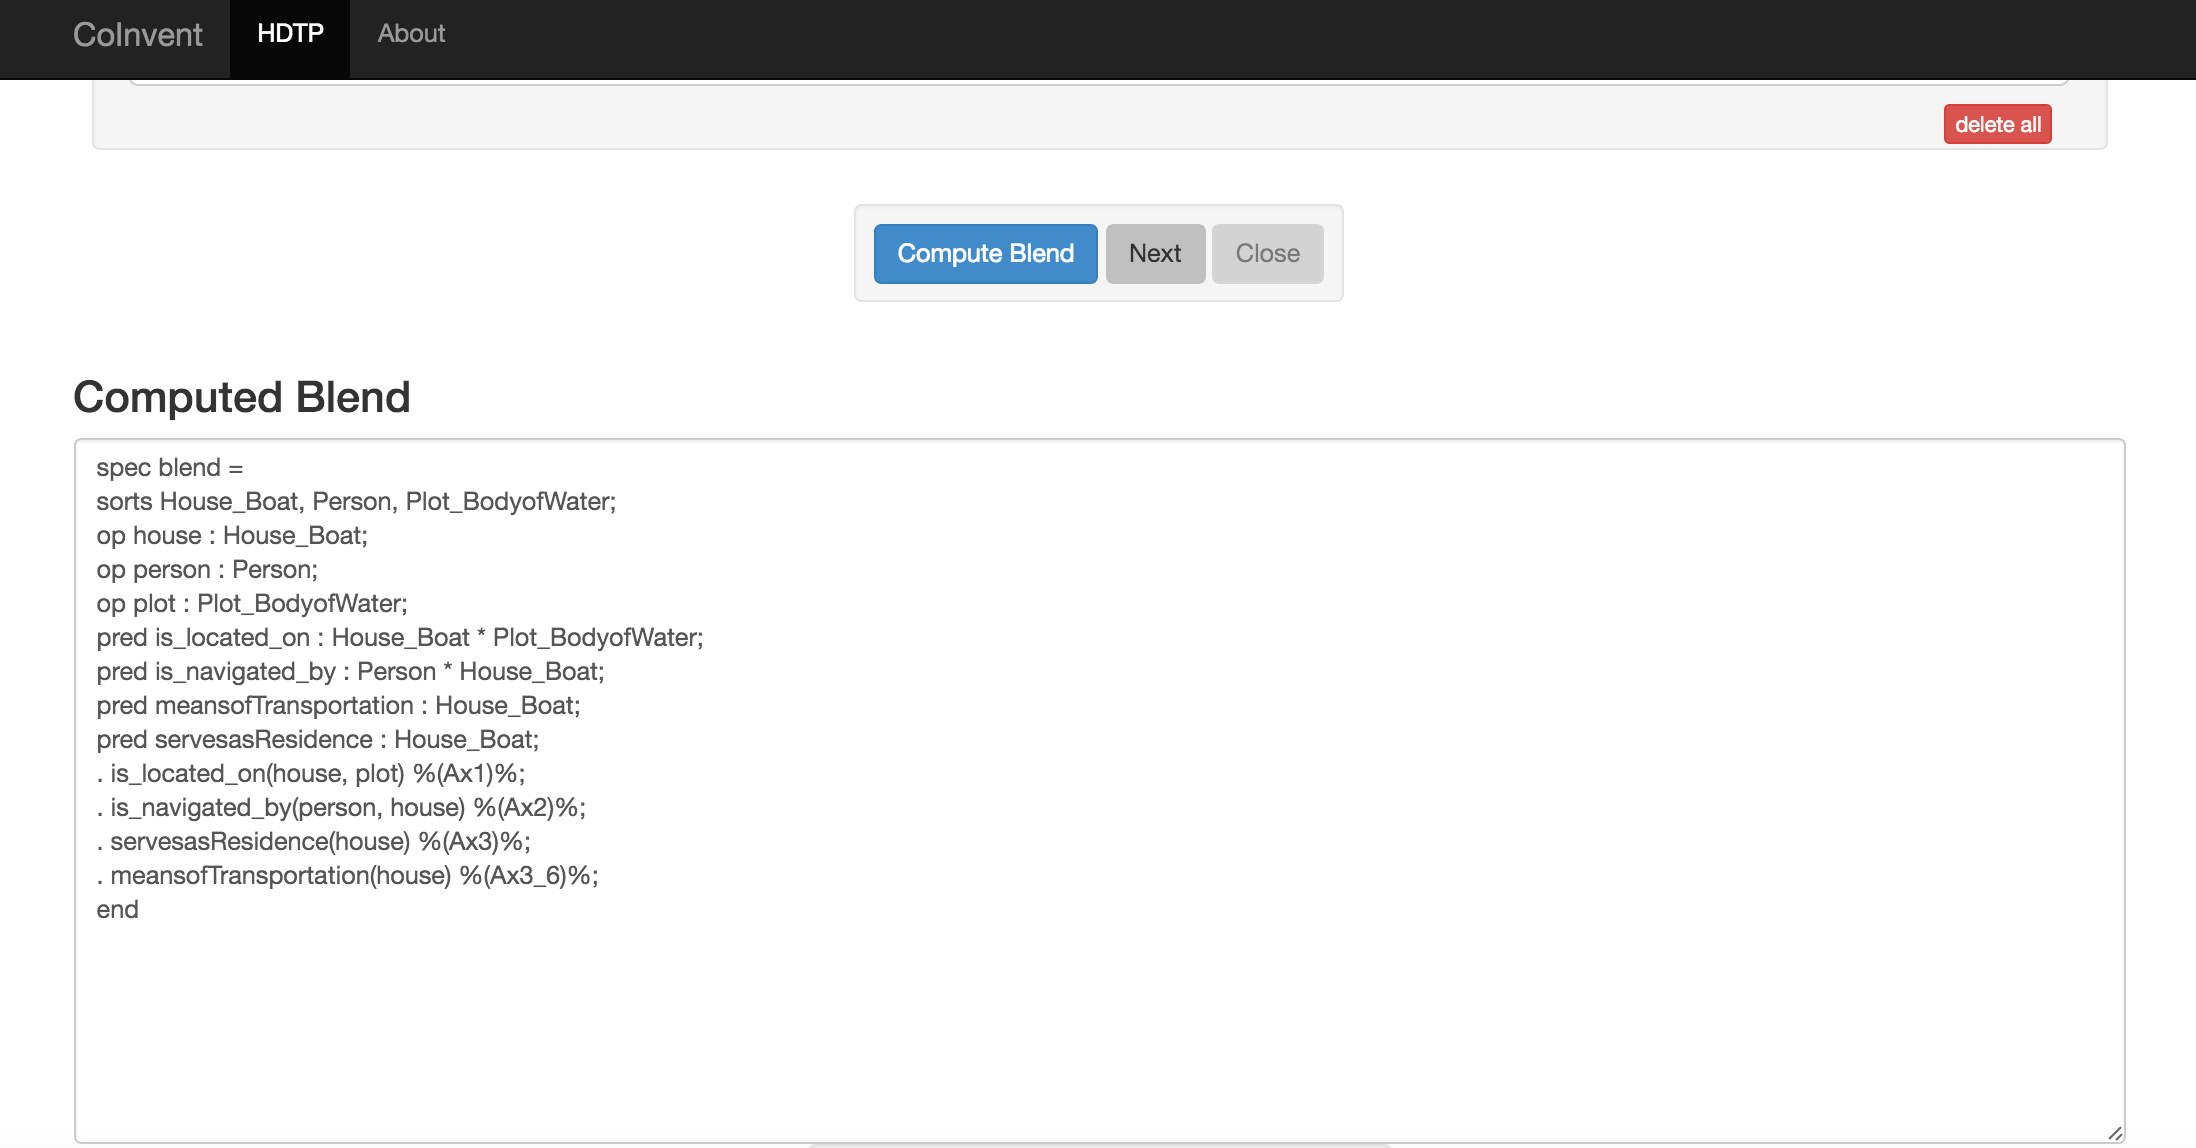
\includegraphics[width=\textwidth]{ss7.png}
\end{center}
\label{fig:ss6}
\caption{Selecting a saved blend as an input theory}
\end{figure}

\begin{figure}[!h]
\begin{center}
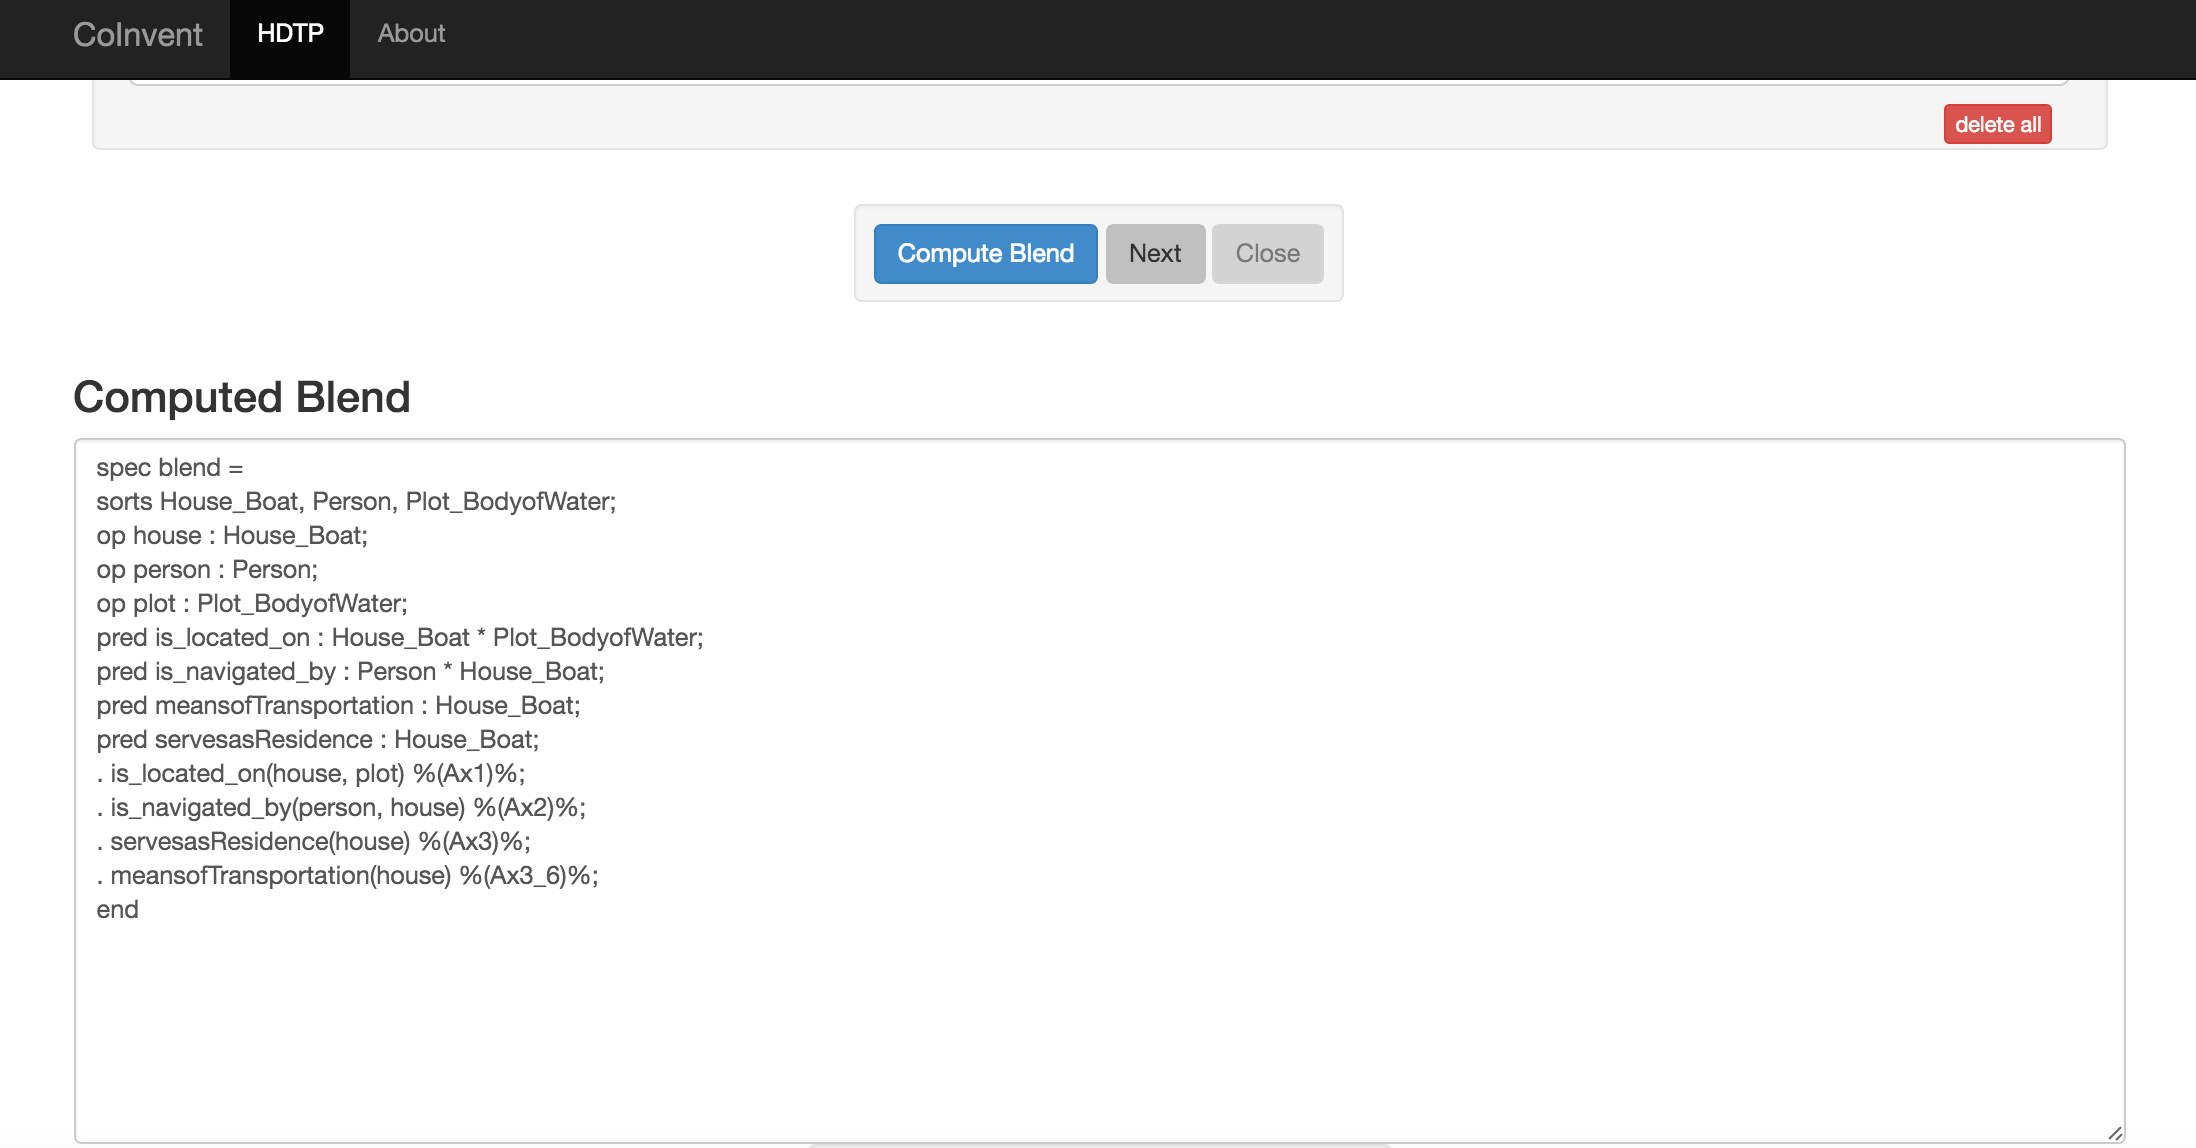
\includegraphics[width=\textwidth]{ss7.png}
\end{center}
\label{fig:ss6}
\caption{Requesting a new answer for the generic space and morphisms from HDTP, and recalculating the blend}
\end{figure}

